\documentclass[10pt]{article}

\usepackage[T1]{fontenc}
\usepackage[utf8]{inputenc}
%\usepackage{beton}
%\usepackage{ccfonts}
%\usepackage{concrete}
\usepackage{concmath}
\usepackage{eulervm}
\usepackage{amsmath,amsthm,amssymb}
\usepackage{mathtools}
\usepackage{multicol}
\usepackage{marginnote}
\usepackage{pgfplots}
\usepackage{float}
\usepackage{hyperref}
\pgfplotsset{compat=1.5}

\usepackage{mathtools}

\usepackage{wasysym}
\usepackage[margin=1.5in]{geometry} 
\usepackage{enumerate}
\index{\usepackage}\usepackage{multicol}

\newcommand{\N}{\mathbf{N}}
\newcommand{\Z}{\mathbb{Z}}

\newcommand{\R}{\mathbf{R}}
\newcommand{\C}{\mathbf{C}}
\newcommand{\Pbb}{\mathbb{P}}
\newcommand{\Fcal}{\mathcal{F}}
\newcommand{\Acal}{\mathcal{A}}
\newcommand{\Ecal}{\mathcal{E}}
\newcommand{\Ebb}{\mathbb{E}}
\newcommand{\Qbb}{\mathbb{Q}}

\newenvironment{theorem}[2][Theorem]{\begin{trivlist}
  \item[\hskip \labelsep {\bfseries #1}\hskip \labelsep {\bfseries #2.}]}{\end{trivlist}}
\newenvironment{lemma}[2][Lemma]{\begin{trivlist}
  \item[\hskip \labelsep {\bfseries #1}\hskip \labelsep {\bfseries #2.}]}{\end{trivlist}}
\newenvironment{exercise}[2][Exercise]{\begin{trivlist}
  \item[\hskip \labelsep {\bfseries #1}\hskip \labelsep {\bfseries #2.}]}{\end{trivlist}}
\newenvironment{reflection}[2][Reflection]{\begin{trivlist}
  \item[\hskip \labelsep {\bfseries #1}\hskip \labelsep {\bfseries #2.}]}{\end{trivlist}}
\newenvironment{proposition}[2][Proposition]{\begin{trivlist}
  \item[\hskip \labelsep {\bfseries #1}\hskip \labelsep {\bfseries #2.}]}{\end{trivlist}}
\newenvironment{corollary}[2][Corollary]{\begin{trivlist}
  \item[\hskip \labelsep {\bfseries #1}\hskip \labelsep {\bfseries #2.}]}{\end{trivlist}}

\newenvironment{definition}[2][Definition]{\begin{trivlist}
  \item[\hskip \labelsep {\bfseries #1}\hskip \labelsep {\bfseries #2.}]}{\end{trivlist}}

\begin{document}
	
  \renewcommand{\qedsymbol}{\smiley}
	\title{Investments Class \\ Problem set 1}
	\author{Daniel Grosu, William Martin, Denis Steffen}
	
	\maketitle

  \begin{exercise}{1}
    First, we need to solve the Geometric Brownian Motion SDE. 
    The SDE is given by: 
    $$ \frac{dS_t}{S_t} = \mu dt + \sigma dz_t$$ where $z_t$ is a standard Brownian Motion. 
    We can apply Itô's lemma on the stochastic process $Y_t = f(S_t) = \ln(S_t)$.
    Thus, $$ dY_t = 0 dt +  \frac{1}{S_t}dS_t + \frac{1}{2}\frac{-1}{S_t^2}(\sigma S_t)^2 dt = \mu dt + \sigma dz_t - \frac{\sigma^2}{2}dt$$
    and $$ \ln(S_t) = (\mu-\frac{\sigma^2}{2})t + \sigma dz_t$$
    The solution of the SDE is: $ S_t = S_0 \exp((\mu-\frac{\sigma^2}{2})t+ \sigma z_t)$.
    Simulating on $10$ years, with the given drift and volatility parameters, the share price can be found in Figure \ref{GMB}. 
    \begin{figure}[h]
      \centering
      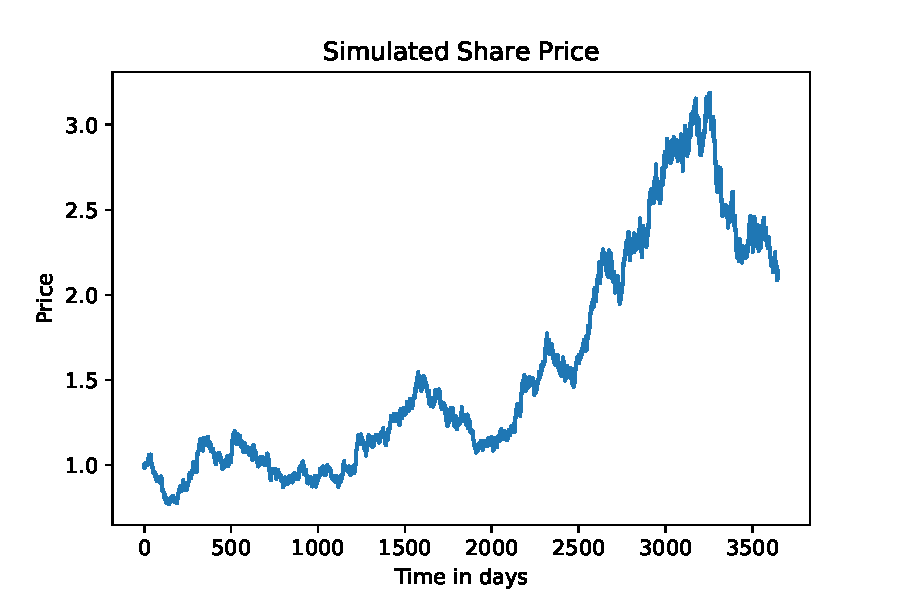
\includegraphics[scale = 0.71]{Figures/simulated.pdf}
      \caption{Geometric Brownian Motion share price simulation}
      \label{GMB}
    \end{figure}
  \end{exercise}



  %\section*{Python Code}

  % \subsection*{Exercise}
  % \lstinputlisting{code/exercise.py}
\end{document}
 